\documentclass[addpoints]{exam}

\usepackage{caption}
\usepackage{graphbox}
\usepackage{hyperref}
\usepackage{multirow}
\usepackage{pythonhighlight}
\usepackage{subcaption}
\usepackage{tabularx}
\usepackage{xcolor}

% Header and footer.
\pagestyle{headandfoot}
\runningheadrule
\runningfootrule
\runningheader{CS 201 Data Structures II}{Homework 1: Lists}{Spring 2023}
\runningfooter{}{Page \thepage\ of \numpages}{}
\firstpageheader{}{}{}

% \qformat{{\large\bf \thequestion. \thequestiontitle}\hfill[\totalpoints\ points]}
\qformat{{\large\bf \thequestion. \thequestiontitle}\hfill}
\boxedpoints
\printanswers

\graphicspath{{images/}}

\newcommand\colheader[1]{\multicolumn{1}{c}{#1}} % Note: no vertical bars

\title{Homework 1: Lists}
\author{CS 201 Data Structures 2\\Habib University}
\date{Spring 2023}

\begin{document}
\maketitle

% This write-up has 3 parts. The first part provides an explanation of your implementation tasks. It refers to code that is provided in the appendices in the third part. The second part lists the tasks for you to do. It contains space for you to enter your solutions to some of the problems. The third part lists code which is referred to in the first part.

% You have to fill in the solutions in the second part, and complete the code files in the accompanying \texttt{src/} folder as described in Part 1. Please work in this file, \texttt{hw1.tex}, and not in a copy. When submitting, please remove the first and third parts from this file.

% \part{Explanation}

% In this assignment, we will implement an \textit{ArrayList} to represent a \textit{List}. We will use the \textit{List} to implement an image and will write operations for the image.

% \section{Image Operations}
% \label{sec:imgops}

% We will work with RGB images and perform four operations on them--channel suppression, rotations, mask application, and resize. None of these operations is \textit{destructive}. That is, the operations do not alter the original image, rather they return a new image containing the result of the operation.

% \subsection{Channel Suppression}

% An image is said to contain color values in different \textit{channels}. In an RGB image, the channels are Red, Blue, and Green. Each channel contains the intensities for that color for every pixel in the image. The values from all three channels at a pixel yield the RGB value at the pixel. A channel suppression operation switches off a specific channel. That is, all intensities in that channel are turned to zero, or turned off. Figure \ref{fig:channel} shows an original image and two modifications, one with the blue channel turned off, and the other with only the blue channel turned on, i.e. the red and green channels turned off.

% \begin{figure}
%   \centering
%   \begin{subfigure}{.3\textwidth}
%     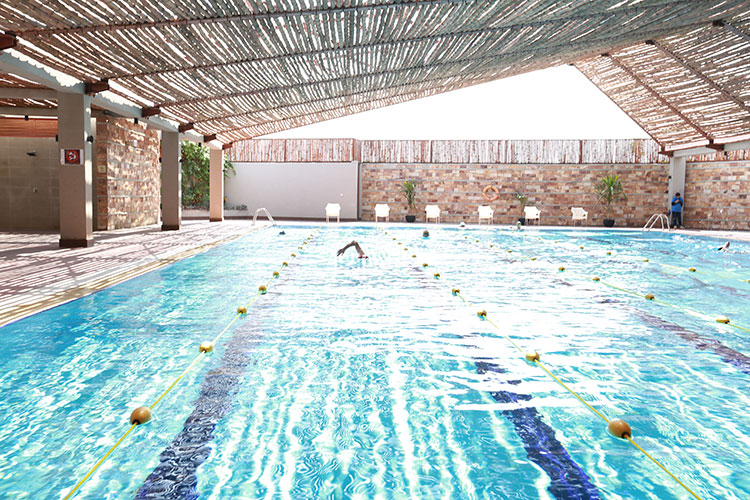
\includegraphics[width=\textwidth]{pool}
%     \caption{An RGB image of a swimming pool.}
%   \end{subfigure}
%   \begin{subfigure}{.3\textwidth}
%     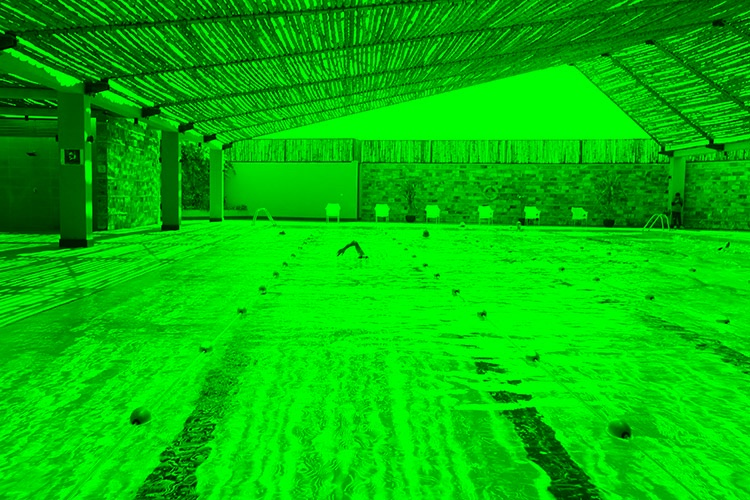
\includegraphics[width=\textwidth]{pool-sans-blue}
%     \caption{The image with the blue channel turned off.}
%   \end{subfigure}
%   \begin{subfigure}{.3\textwidth}
%     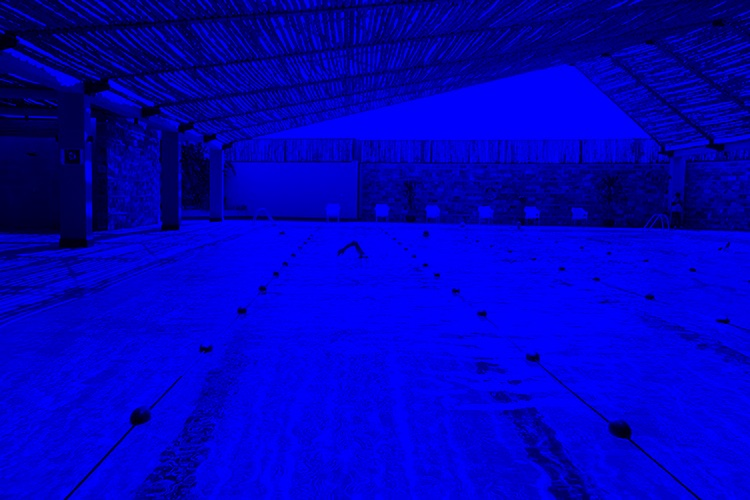
\includegraphics[width=\textwidth]{pool-only-blue}
%     \caption{The original image with only the blue channel turned on.}
%   \end{subfigure}
%   \caption{Example of channel suppression.}
%   \label{fig:channel}
% \end{figure}

% \subsection{Rotation}

% Given a square image, i.e. one whose width is equal to its height, this operation generates a new image that contains rotations of the original image. Figure \ref{fig:rotate} shows an example of applying the operation. The resulting image has twice the dimensions of the original image, i.e. twice the width and twice the height. It contains 4 appropriately placed sub-images which, going anti-clockwise are the original image rotated anti-clockwise by increments of  $90^\circ$.

% \begin{figure}
%   \centering
%   \begin{subfigure}{.2\textwidth}
%     
\includegraphics[scale=.5]{hu-logo}
%     \caption{A square image.}
%   \end{subfigure}
%   \begin{subfigure}[c]{.35\textwidth}
%     
\includegraphics[scale=.5]{hu-logo-rotated}
%     \caption{The image obtained as a result of applying rotations to the original image.}
%   \end{subfigure}
%   \caption{Example of rotation.}
%   \label{fig:rotate}
% \end{figure}

% \subsection{Applying a Mask}

% A \textit{mask} specifies certain \textit{weights} and applying the mask to an image entails replacing the value at each pixel in the image with a \textit{weighted sum} or \textit{weighted average} of the values of its \textit{neighbors}. The weights and the neighbors to consider for the average are specified by the mask.

% A mask is an $n \times n$ array of integers representing weights. For our purposes, $n$ must be odd. This means that the $n \times n$ array has a well defined center--the \textit{origin}. The weights in the mask can be arbitrary integers--positive, negative, or zero.

% For each pixel in the input image, think of the mask as being placed on top of the image so its origin is on the pixel we wish to examine. The intensity value of each pixel under the mask is multiplied by the corresponding value in the mask that covers it. These products are added together. Always use the original values for each pixel for each mask calculation, not the new values that you compute as you process the image.

% For example, refer to Figure \ref{fig:mask-full}, which shows the  $3 \times 3$ mask,
% \[
%   \left[
%     \begin{array}{ccc}
%       1 & 3 & 1 \\
%       3 & 5 & 3 \\
%       1 & 3 & 1 \\
%     \end{array}
%     \right]
% \]
% and an image on which we want to perform the mask computation. Suppose we want to compute the result of the mask computation for pixel $e$. This result would be:
% \[
%   a + 3b + c + 3d + 5e + 3f + g + 3h + i
% \]
% Some masks require a \textit{weighted average} instead of a weighted sum. The weighted average in the case of Figure \ref{fig:mask-full} for pixel $e$ would be:
% \[
%   \frac{a + 3b + c + 3d + 5e + 3f + g + 3h + i} {1 + 3 + 1 + 3 + 5 + 3 + 1 + 3 + 1}
% \]
% Instead of doing this calculation for each channel individually at a pixel, for the purpose of this calculation, replace the value of each channel at the pixel with the average channel value at the pixel. For example, if the pixel is given by $(r, g, b) = (107, 9, 218)$, then apply the mask to the average value $(107 + 9 + 218)//3 = 111$ (integer division) and copy the result to each channel of the corresponding pixel in the output image. This effectively converts the output image to grayscale.

% Note that sometimes when you center the mask over a pixel, the mask will hang over the edge of the image. In this case, compute the weighted sum of only those pixels that the mask covers. For the example shown in Figure \ref{fig:mask-hang}, the weighted sum for the pixel $e$ is given by:
% \[
%   3b + c + 5e + 3f + 3h + i
% \]
% and the weighted average is as follows.
% \[
%   \frac{3b + c + 5e + 3f + 3h + i}{3+1+5+3+3+1}
% \]
% Integer division is used when computing averages in order to ensure that pixel intensities are integers.

% \begin{figure}
%   \centering
%   \begin{subfigure}{.48\textwidth}
%     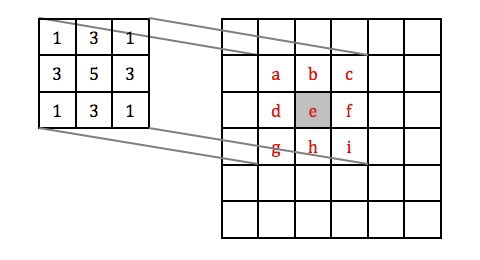
\includegraphics[width=\textwidth]{mask1}
%     \caption{Overlay the $3 \times 3$ mask over the image so it is centered on pixel $e$ to compute the new value for pixel $e$.}\label{fig:mask-full}
%   \end{subfigure}
%   \begin{subfigure}[c]{.48\textwidth}
%     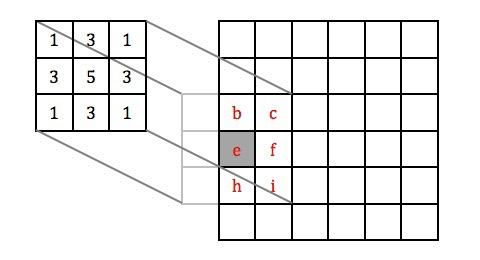
\includegraphics[width=\textwidth]{mask2}
%     \caption{If the mask hangs over the edge of the image, use only those mask values that cover the image in the weighted sum.}\label{fig:mask-hang}
%   \end{subfigure}
%   \caption{Applying a mask to an image.}
%   \label{fig:mask}
% \end{figure}

% \subsubsection{Applications of Masks}

% Applying different masks leads to different properties. For example, applying the following mask leads to blurring of the image. Figures \ref{fig:mask-orig} and \ref{fig:mask-blur} show the blurring effect of this mask. Note that color information is lost as mentioned above.
% \[
%   \left[
%     \begin{array}{ccccc}
%       2 & 4  & 5  & 4  & 2 \\
%       4 & 9  & 12 & 9  & 4 \\
%       5 & 12 & 15 & 12 & 5 \\
%       4 & 9  & 12 & 9  & 4 \\
%       2 & 4  & 5  & 4  & 2 \\
%     \end{array}
%     \right].
% \]

% Another application we use is an implementation of \textit{Canny Edge Detection} using \textit{Sobel Operators}. Once the image has been blurred as above, two more \textit{filters}, or masks, (the Sobel operators) are applied in succession to the blurred image. These filters determine the change in intensity, which approximates the horizontal and vertical derivatives.
% \[
%   G_x =   \left[
%     \begin{array}{ccc}
%       -1 & 0 & 1 \\
%       -2 & 0 & 2 \\
%       -1 & 0 & 1
%     \end{array}
%     \right], \quad
%   G_y =   \left[
%     \begin{array}{ccc}
%       -1 & -2 & -1 \\
%       0  & 0  & 0  \\
%       1  & 2  & 1
%     \end{array}
%     \right].
% \]
% After these operations are applied one after the other to the blurred image, the values obtained are used to search for edges based on the magnitude and direction of the change in intensity. An example of the final result is shown in Figure \ref{fig:mask-edge}.

% \begin{figure}
%   \centering
%   \begin{subfigure}{.31\textwidth}
%     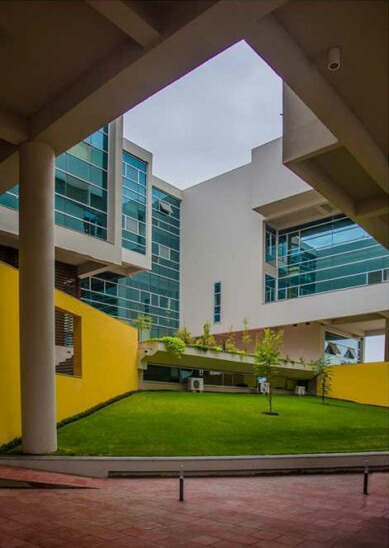
\includegraphics[width=\textwidth]{campus}
%     \caption{An image with sharp details and several lines.}\label{fig:mask-orig}
%   \end{subfigure}
%   \begin{subfigure}[c]{.31\textwidth}
%     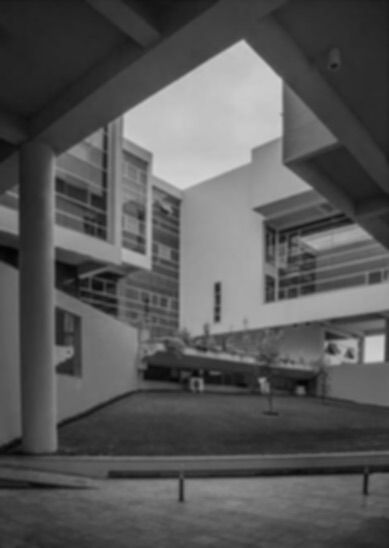
\includegraphics[width=\textwidth]{campus-blur}
%     \caption{Result of applying the blur mask to the original image.}\label{fig:mask-blur}
%   \end{subfigure}
%   \begin{subfigure}[c]{.31\textwidth}
%     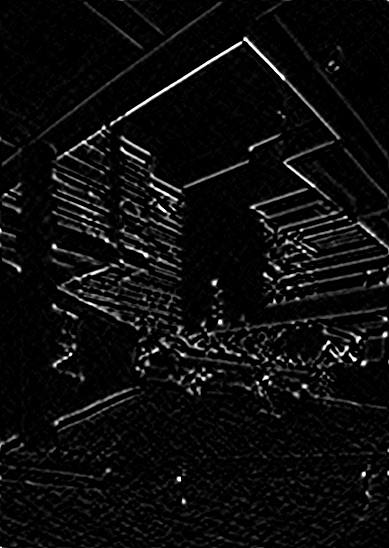
\includegraphics[width=\textwidth]{campus-edge-detect}
%     \caption{Result of applying the Sobel filters to the blurred image.}\label{fig:mask-edge}
%   \end{subfigure}
%   \caption{Blurring and detection of edges in an image using masks.}
%   \label{fig:mask-apply}
% \end{figure}

% \subsection{Resize}

% Given an image, this operation generates a new image that has twice the dimensions of the original image i.e, twice the width and twice the height.
% Figure \ref{fig:resize} shows a 4x3 image which is resized to twice its size. The resized image has 4 times as many pixels and some of them take on the values from the original image as shown. For the pixels shown to be blank, color values are not known and have to be computed from the known values.
% Consider the labeled pixels in the resized image below. One way to fill in the missing color information is as follows.
% \[
%   P = \frac{1}{2}(A + B),\; T = \frac{1}{2}(C + D),\; Q = \frac{1}{2}(A + C),\; S = \frac{1}{2}(B + D)
% \]
% There are various ways to compute R, all of which are ultimately equivalent.
% \[
%   R = \frac{1}{2}(P + T) = \frac{1}{2}(S + Q) =  \frac{1}{4}(A + B + C + D) = \frac{1}{4}(P + Q + S + T) = \frac{1}{8}(A + B + C + D + P + Q + S + T)
% \]
% The boundary pixels pose a problem as some of the neighboring pixels required for the average do not exist. In such cases, only the existing neighbors are used for the average.

% Notice how all the above expressions are affine combinations. Furthermore, the colors for P, Q, S, and T are \textit{linearly interpolated} from their horizontal or vertical neighbors. The color for R is a \textit{bilinear interpolation}: it is a linear interpolation of P and T, or Q and S, which are themselves linear interpolations.

% \begin{figure}
%   \centering
%   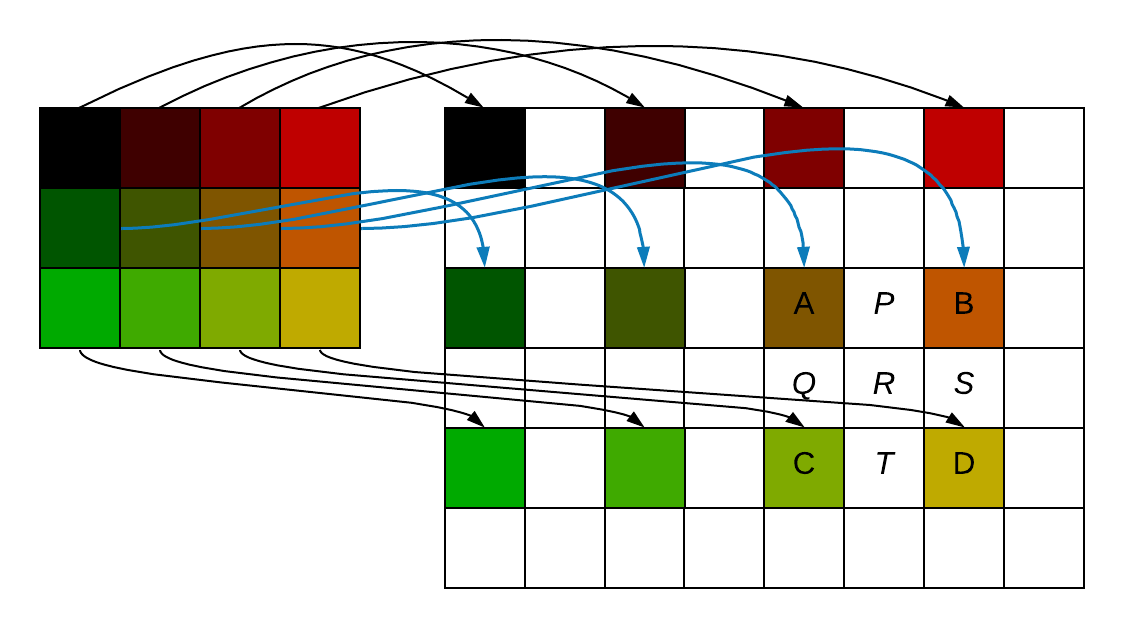
\includegraphics[width=.4\textwidth, align=t]{resize}
%   \caption{Bilinear Interpolation}
%   \label{fig:resize}
% \end{figure}
% \underline{Note}: All divisions in the above expressions are integer divisions.

% \section{Image}

% We treat an image as a grid of \textit{pixels} where each pixel is represented as an RGB value indicating the red, green, and blue intensities of the pixel. An image has \textit{dimensions}, namely \textit{width} and \textit{height}, which determine the number of \textit{rows} and \textit{columns} in the image. Every pixel in the image is at a unique combination of row and column numbers which can therefore be used as a coordinate system in the image. An image with width $w$ and height $h$ is said to be of size $w\times h$. Figure \ref{fig:img-dim} shows the column and row numbers in a $w\times h$ image along with the resulting pixel coordinates. Note that the coordinate is just a means to locate a pixel in the image, it is not the value stored at the pixel. The value stored at a pixel is a triplet denoting the red, green, and blue intensities respectively.

% We will work with a \textit{flattened} representation of an image. That is, we will store the pixel values in a 1-dimensional list structure as opposed to a 2-dimensional structure (programming languages generally store multi-dimensional arrays in their flattened form) . The list stores pixel values as they appear in the image from left to right and top to bottom. Figure \ref{fig:img-rgb} shows a $5\times 5$ image with some supposed RGB values. Note that each value would be a triplet of integers, each integer between 0 and 255 inclusive. Using our representation, the image in Figure \ref{fig:img-rgb} will be represented as the list:
% \[
%   [a, b, c, d, e, f, g, h, i, j, k, l, m, n, o, p, q, r, s, t, u, v, w, x, y]
% \]

% \begin{figure}
%   \begin{subfigure}{.65\textwidth}
%     \small
%     \begin{tabular}{c*{6}{c|}}
%                                                       & \colheader{} & \multicolumn{5}{c}{Columns}                                                                            \\
%       \colheader{}                                    & \colheader{} & \colheader{0}               & \colheader{1} & \colheader{2} & \colheader{\ldots} & \colheader{$(w-1)$} \\\cline{3-7}
%       \multirow{4}{*}{\rotatebox[origin=c]{90}{Rows}} & 0            & $(0, 0)$                    & $(0, 1)$      & $(0, 2)$      & $\ldots$           & $(0, w-1)$          \\\cline{3-7}
%                                                       & 1            & $(1, 0)$                    & $(1, 1)$      & $(1, 2)$      & $\ldots$           & $(1, w-1)$          \\\cline{3-7}
%                                                       & 2            & $(2, 0)$                    & $(2, 1)$      & $(2, 2)$      & $\ldots$           & $(2, w-1)$          \\\cline{3-7}
%                                                       & \vdots       & \vdots                      & \vdots        & \vdots        & $\ddots$           & \vdots              \\\cline{3-7}
%                                                       & $(h-1)$      & $(h-1, 0)$                  & $(h-1, 1)$    & $(h-1, 2)$    & $\ldots$           & $(h-1, w-1)$        \\\cline{3-7}
%     \end{tabular}
%     \caption{Row and column numbers of an image with width $w$ and height $h$. Pixel coordinates are also shown.}\label{fig:img-dim}
%   \end{subfigure}
%   \begin{subfigure}{.3\textwidth}
%     \[
%       \begin{array}{|*{5}{c|}}
%         \hline
%         a & b & c & d & e \\\hline
%         f & g & h & i & j \\\hline
%         k & l & m & n & o \\\hline
%         p & q & r & s & t \\\hline
%         u & v & w & x & y \\\hline
%       \end{array}
%     \]
%     \caption{A $5\times 5$ image with supposed pixel values.}\label{fig:img-rgb}
%   \end{subfigure}
%   \caption{Image dimensions and pixel coordinates.}
%   \label{fig:img}
% \end{figure}
% \newpage
% \section{Implementation Details and Tasks}

% We will be working with a \pyth{MyImage} class as shown in Listing \ref{lst:img} on Page \pageref{lst:img}, also included in the accompanying file \texttt{src/myimage.py}. Its implementation is complete but requires a concrete implementation of \pyth{MyList} which is our implementation of the \textit{List} interface. The implementation to be used is specified in the constructor of \pyth{MyImage}.

% An implementation of \pyth{MyList} is shown in Listing \ref{lst:lst} on Page \pageref{lst:lst}, also included in the accompanying file \texttt{src/mylist.py}. The implementation is mostly complete except for the segments marked as \pyth{pass}. These are to be implemented appropriately in the subclasses of \pyth{MyList} which are indicated at the end of the listing and whose implementation is completely missing. Writing their implementations is one of your tasks in this assignment.

% Once you are done implementing \pyth{MyList} subclasses, the \pyth{MyImage} class is ready to be operated on. Functions corresponding to the operations described in Section \ref{sec:imgops} are shown in Listing \ref{lst:imgops} on Page \pageref{lst:imgops} and included in the accompanying file \texttt{src/image\_operations.py}. None of the operations is destructive. That is, each operates on a \pyth{MyImage} instance and returns the result as a new \pyth{MyImage} instance. The functions are missing implementations. Writing their implementations is another of your tasks in this assignment.

% \subsection{Tasks}
% \label{sec:tasks}

% \begin{itemize}
%   \item Go over the provided files thoroughly in order to understand what they do or are expected to do.
%   \item Provide implementations for unimplemented methods, i.e. those that have \pyth{pass} in their body.
%   \item Derive \pyth{ArrayList} class  from \pyth{MyList} and provide its implementation in the same file. \pyth{ArrayList} implements the list using \href{https://www.programiz.com/python-programming/array}{python arrays}.
% \end{itemize}

% \subsection{Requirement}

% You will need to install \href{https://pillow.readthedocs.io/en/5.3.x/index.html}{Pillow} which will prove the \pyth{PIL} module used in the provided code.

% \subsection{Tips}

% Below are some tips to avoid the errors that have previously caused tests to fail. Following these may save you many frustrating hours of debugging!
% \begin{itemize}
%   \item Delay division as much as possible and perform \pyth{int} division wherever needed.
%   \item When writing gray values to file, make sure to clamp them to [0,255].
%   \item Take care about imagine indexing.
%   \item Be careful when creating a copy of the image. Use the copy where needed and the original where needed.
%   \item Do not forget to average the RGB values when the corresponding flag in \pyth{apply_mask} is enabled.
%   \item Take care about efficiency. Some structures are slow. If, on top, your code is inefficient, the automated tests may fail due to time out.
  
% \end{itemize}

% \subsection{Testing}

% Once you have successfully implemented the subclasses and image operations, you can test your code by creating an image and performing operations on it. Your submission will be tested automatically by GitHub using the accompnaying \pyth{pytest} file, \texttt{test\_image.py}.


% \section{Credits}

% This homework is adapted from Homework 3 of the Fall 2014 offering of 15-122: Principles of Imperative Computation at Carnegie Mellon University (CMU).

% % ''' Python debugging: https://realpython.com/python-debugging-pdb/
% % '''

% \part{Problems}

% The grading is defined in the accompanying rubric file.
\begin{questions}
  % \titledquestion{Implementation} Complete the tasks listed in Section \ref{sec:tasks} by providing the implementations in the indicated files.


  \titledquestion{Amortized Analysis}
  Consider an \pyth{ArrayStack} implementation of the \pyth{List} interface with a slightly altered \pyth{resize()} operation. Instead of reserving space for $2n$ elements in the new array, it reserves space for $n + \lceil \frac{n}{4} \rceil$ elements. Prove that the \pyth{append()} operation still takes $O(1)$ time in the amortized sense.
  \begin{solution}
    \newline
    Let's assume we have to perform the append operation n times. 
    Let the cost of each append operation be $x_i$, while the size of the array after each append operation be $l_i$. 
    \newline
    \newline
    We want to prove that the append() operation still takes O(1) time in the amortized sense even if it reserves space for $n + \lceil \frac{n}{4} \rceil$ elements instead of $2n$ elements.
    That means that if we apply the append operation n times, our total cost would be $O(n)$
    \newline
    \newline
    The total cost of resizing is calculated by adding the cost every time resize operation is performed, i.e. the size goes from $l_i$ (which is our current size) to $l_{i+1}$ (which is our size after resize operation is performed), to total.  Here, $l_i$ is $k \cdot \frac{n}{4}$ where $k$ is a positive integer
    \newline
    \newline
    Using the equation for new array size (after resizing operation is performed):
    \newline
    \newline
    $l_{i+1} = n + \left\lfloor \frac{l_i}{4} \right\rfloor$
    \newline
    \newline
    Since $l_i$ is $k \cdot \frac{n}{4}$, substituting it in the equation $l_{i+1} = n + \left\lfloor \frac{l_i}{4} \right\rfloor = n + \left\lfloor \frac{k \cdot \frac{n}{4}}{4} \right\rfloor = n + \left\lfloor \frac{k}{4} \right\rfloor \cdot \frac{n}{4}$
    \newline
    \newline
    Because $k$ is a positive integer, $\left\lfloor \frac{k}{4} \right\rfloor \cdot \frac{n}{4} < \left\lfloor \frac{k}{4} \right\rfloor \cdot \frac{n}{4} + \frac{1}{4} \cdot \frac{n}{4}$.
    \newline
    \newline
    Therefore, $l_{i+1} < n + \frac{n}{4} \cdot \left(\frac{k}{4} + 1\right)$.
    \newline
    \newline
    This shows that the size of array after resize operation $ < n + \frac{n}{4}$ always. Hence, the total resize operations cost $ = O(n)$.
    \newline
    \newline
    The cost every time append operation peformed $x_i =  1$. Therefore, the total cost which is the cost of this operation performed $n$ times would be $O(n)$. This is the cost for one resize operation, i.e. the size goes from $l_i$ to $l_{i+1}$.
    \newline
    \newline
    The total cost for all resize operations would be the sum of the cost of each of the resize operation, i.e. $O(n) + O(n) = O(n)$. Therefore, the the average cost per append operation is $O(1)$.
    


  \end{solution}

\end{questions}

% \newpage
% \part{Appendices}

% \appendix
% \section{\pyth{MyImage}}
% \lstinputlisting[style=mypython, frame=single, caption=Image Type, label={lst:img}]{src/myimage.py}

% \newpage
% \section{\pyth{MyList}}
% \lstinputlisting[style=mypython, frame=single, caption=List Type, label={lst:lst}]{src/mylist.py}

% \newpage
% \section{Image Operations}
% \lstinputlisting[style=mypython, frame=single, caption=Image Operations, label={lst:imgops}]{src/image_operations.py}



\end{document}

%%% Local Variables:
%%% mode: latex
%%% TeX-master: t
%%% End:
